\chapter{Domain Specific Languages}

Software Frameworks and Domain Specific Languages are related in the sense 
that both aim to support the construction of specific types of software application. 
In many ways you can view the essence of a DSL as a software framework. 
Super-languages must support he definition of DSLs through language extension
facilities.

This chapter describes the relationship between a Software Framework and
a DSL. It gives an example of a DSL based on that of Martin Fowler from 
his presentation at JAOO 06.

\section{Software Frameworks and Domain Specific Languages}

Domain Specific Languages are increasingly popular as a technology 
and an approach to constructing applications. The idea is that a specific 
aspect of an application can be supported through the design and use of a 
language. The language may be used to configure parts of the application, 
to describe the GUI, to encode processing rules etc. Proponents of DSLs 
claim that, since the language abstracts away from the implementation 
details of the code otherwise necessary to achieve the same effect, the 
overall quality of the process and product is increased. The aspect 
supported by the DSL is easier to implement, the development is less 
error prone (since the language is specifically designed to support the task), 
the debugging and maintenance of the application is easier.

A Software Framework is a collection of classes that capture a design 
pattern or an aspect of an application. The key feature of a software 
framework is that it represents a reusable component where some of the 
features of the framework are fixed in structure and behaviour and some 
are left open to extension by the user. A framework differs from a more 
traditional software library in that the user provides the framework with 
the implementation of services that the framework calls. In a software 
library this works the other way round where the user calls services 
provided by the library (the so-called {\em Inversion of Control}). There 
are many examples of large scale general purpose software frameworks, 
such as Eclipse, but many packages provided for OO languages can be 
thought of as frameworks. Frameworks are also an architectural design pattern.

Domain specific languages usually (but not always) {\em do something}. To 
achieve this, the language has a semantics (a description of how it 
should operate) and some means of implementing the semantics - a DSL 
engine. The DSL engine is supplied with a representation of programs in 
the DSL. This program-as-data is then processed by the engine to achieve 
the required task.

A DSL engine is exactly the same as a Software Framework. The engine 
expects to be supplied with an implementation of a specific collection of 
services {\em implemented as data}. The task of the framework is to perform some 
standard, albeit domain specific, processing which uses the services 
supplied as DSL programs when appropriate.

It is a fact of Software Engineering that anything you can implement 
in program code, you can also implement in data with an associated 
engine that processes the data. This is exactly the relationship between 
Software Frameworks and DSLs. But why would you implement the services 
as data rather than implement them directly as program code (for example 
as an implementation of an abstract method or an interface)?

The answer is fundamentally an issue of {\em quality}. By pushing more of the 
framework services into data, the framework increases its level of control  
- nothing can escape! Therefore the more the framework matures, the higher 
the quality of the applications that use it. Data can also be processed in 
many ways: checking it, repairing it, translating it. This level of control 
over the services is not available to frameworks that represent their information 
as program code.

There are differences between a Software Framework and a DSL. Typically, a 
DSL will have some {\em concrete syntax} which is used to express the data to be 
supplied to the engine. Frameworks do not tend to have specific language 
syntax - they use a general purpose programming language to construct the 
services. However, these differences are not as significant as they might 
appear at first.

A DSL is usually implemented in terms of a parser that translates the 
concrete syntax into the abstract syntax (the data structures) and then 
an engine that processes the abstract syntax (the framework). The essence 
of the DSL is the abstract syntax and the engine - after all that is the 
part which is doing all the real work. The concrete syntax just makes the 
DSL easy to use and there may be many concrete syntaxes for the same DSL. 
Therefore, the {\em essence} of a DSL is the data and the engine - a Software 
Framework!

The rest of this document drills into the view of DSL as Software Framework. 
We use a simple example application to illustrate some of the points. The 
example (in addition to the link to Software Frameworks) is taken from a talk 
given by Martin Fowler at JAOO 06.

\section{Example Application}

Suppose we have data that contains information about customer events. 
A customer event might be a service call including the name of the customer, 
the type of the call (failed hardware, billing query etc) and the date. This 
information may be provided in real-time or in a log file as text:
\begin{lstlisting}
SVCLFOWLER    10101MS0120050313
SVCLHOHPE    10201DX0320050315
SVCLTWO     x10301MRP220050329
USGE10301TWO     x50214..7050329
\end{lstlisting}
The requirement is to have a Java program that processes the information. 
Obviously the first task of the Java application is to split the input 
strings up in terms of their fields. If there are a very small number of 
types of call then it would be OK to just write the appropriate string 
manipulation calls on the input.

However, this will rapidly become tedious and error prone as the number 
of different types of call grows. This leads to the idea of replacing 
the repeating patterns in the code with a software framework. Service 
plug-points in the framework allow the developer to register different 
types of call and the associated string manipulation that goes with it. 
This might be done using an abstract class:
\begin{lstlisting}
framework.registerStrategy(new ReaderStrategy() {
  
  public boolean recognizes(String s) {
    return hasPrefix(s,"SVCL");
  }

  public Record extract(String s) {
    return new ServiceCall(s.subString(4,18),...);
  }
});
\end{lstlisting}
The framework is responsible for processing the raw input text and calling 
the various registered recognizers in order to process the lines.

In developing a framework such as that shown above, we observe that the 
services are written in Java. There is little the framework can do to 
analyze each registered service in order to make sure that it is legal. 
Rules governing a well-formed service might include checking that the 
indices used to chop up the string are non-conflicting and that the prefix 
labels for all recognizers are unique.

In addition to the quality control objections raised above, the service-as-code 
implementation uses a great deal of Java which is standard for each of the 
recognizers. Essentially, there is a pattern to defining a recognizer where 
only the prefix name, the type of the record and indices change. It would be 
much better from the point of quality to be able to abstract away from this 
{\em implementation noise}.

It would be much better to represent the framework services as data. This is 
because the framework can perform analysis on the well-formedness of the 
services and also because data representations of services provides scope 
for concrete syntax which will address the problems that arise from repeating 
boilerplate code.

Fowler gives a service representation something like the following:
\begin{lstlisting}
public void ConfigureCallReader(Framework framework) {
  framework.registerStrategy(ConfigureServiceCall());
  framework.registerStrategy(ConfigureUsage());
}
 
private ReaderStrategy ConfigureServiceCall() {
  ReaderStrategy result = new ReaderStrategy("SVCL",typeof(ServiceCall));
  result.addFieldExtractor(4,18,"CustomerName"));
  result.addFieldExtractor(19,23,"CustomerID"));
  result.addFieldExtractor(24,27,"CalltypeCode"));
  result.addFieldExtractor(28,35,"DataOfCallString"));
}
 
private ReaderStrategy ConfigureUsage() {
  ReaderStrategy result = new ReaderStrategy("USGE",typeof(Usage));
  result.addFieldExtractor(4,8,"CustomerID"));
  result.addFieldExtractor(9,22,"CustomerName"));
  result.addFieldExtractor(30,30,"Cycle"));
  result.addFieldExtractor(31,36,"ReadDate"));
}
\end{lstlisting}
Notice how everything about the service is now represented as data that 
is supplied to the framework. The framework has a model of this language 
(the classes for ReaderStrategy, FieldExtractor etc) that it can manipulate 
the 'program' against. Therefore it can perform analysis on the registered 
services and translate them into something else if it wishes. Neither of 
these activities would be possible of the services were supplied as code.

Finally, note that the services-as-data example above involves further 
boilerplate code. In some ways this is worse than the boilerplate in the 
services-as-code example since there is more of it! Furthermore, we are 
dealing with two languages here: Java is used to represent a language for 
reader strategies. It is therefore difficult to see the wood for the trees.

The solution is to design a concrete syntax for the call language and to 
have a parser translate the concrete syntax into instances of the abstract 
syntax (classes ReaderStrategy, FieldExtractor etc). There can be any number 
of concrete syntaxes for a language. Fowler proposes both XML and a bespoke 
syntax.

XML is popular because it is standard. Whilst XML is widely used for 
configuring tools and frameworks, it is in many ways a lowest common 
denominator and lacks the variety of syntax features that is the essential 
reason for using a concrete syntax in the first place. Having said that, 
XML might be attractive because it can be processed easily by several tools. 
A suitable representation for the DSL described above is:
\begin{lstlisting}
<ReaderConfiguration>
  <Mapping code='SVCL' targetClass='ServiceCall'>
    <Field name='CustomerName' startPos='4' endPos='18'/>
    ...
  </Mapping>
  <Mapping code='USGE' targetClass='Usage'>
    ...
  </Mapping>
  <Strategy>
    <ref name='SVCL'/>
    ...
  </Strategy>
</ReaderConfiguration>
\end{lstlisting}
A bespoke syntax for a DSL should be designed for readability and therefore 
to aid development and maintainability. Here is a possible syntax:
\begin{lstlisting}
@Reader CallReader

  map(SVCL,ServiceCall)
    4-18:CustomerName
    19-23:CustomerID
    24-27:CallTypeCode
    28-35:DataOfCallString
  end

  map(USGE,Usage)
    4-8:CustomerID
    9-22:CustomerName
    30-30:Cycle
    31-36:ReadDate
  end

  do 
    ServiceCall
    Usage
end
\end{lstlisting}

\section{Abstract Syntax}

\begin{figure}
\begin{center}
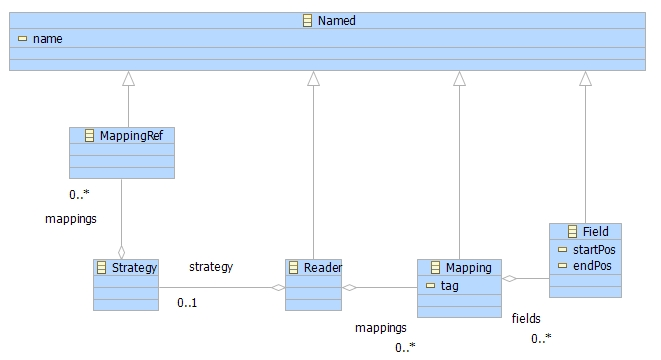
\includegraphics[width=12cm]{LanguageEngineering/DSLs/Images/Readers}
\caption{DSL Abstract Syntax\label{fig:DSLAbstractSyntax}}
\end{center}
\end{figure}

Our DSL requires an abstract syntax to represent the information 
that is supplied to the framework. Figure \ref{fig:DSLAbstractSyntax} shows 
classes and relationships defined by the abstract syntax.The rest of this 
section discusses how these classes are used in the definition of a reader.

Named is an abstract class that defines a name of type string. A Reader 
is a container of mappings and a strategy. The mappings define the tagged 
and formatted fields that are received as input from the log file. Each 
Mapping is named and collectively they define a library available to the 
containing reader reader. The Strategy is used to reference mapping by name. 
The strategy is used to register mappings with the framework. In a more 
sophisticated language, the strategy could impose constraints on how the 
mappings are used, for example by requiring them to be used in a particular 
order.

\section{Implementation}

There are a number of ways in which we can implement the relationship 
between the abstract syntax defined in the previous section and the 
software framework. Two standard ways of achieving this are: to embed 
the language into the same platform as the framework; or, to translate 
the syntax onto a different platform. There is no real reason why you 
would do one rather than the other. In many cases it will be determined 
by other factors, for example when the DSL implementation technology is 
different from the framework technology.

\subsection{Embedded}

Suppose that the technology platform used to represent the DSL is the 
same as that for the framework. In this case we may choose to dynamically 
link the syntax to the framework which will allow new reader definitions 
to be added while the framework is running. Suppose that the framework is 
implemented in XMF and that the class Framework implements a register 
operation:
\begin{lstlisting}
context Framework
  @Operation register(reader:Reader) 
    reader.strategy().register(self,reader)
  end

context Strategy
  @Operation register(framework:Framework,reader:Reader)
    @For ref in mappings do
      ref.register(framework,reader)
    end
  end

context MappingRef
  @Operation register(framework:Framework,reader:Reader)
    reader.getMapping(name).register(framework)
  end

context Mapping
  @Operation register(framework:Framework)
    let r:ReaderStrategy = ReaderStrategy(tag,typeof(name)
    in framework.registerStrategy(r);
       @For field in fields do
         field.register(r)
       end
    end
  end

context Field
  @Operation register(readerStrategy:ReaderStrategy)
    readerStrategy.addFieldExtractor(startPos,endPos,name)
  end
\end{lstlisting}

\subsection{Translational}

If the DSL is implemented in a different technology to the DSL 
or if you wish to impose a phase distinction between the definition-time 
(processing the DSL) and run-time (running the framework) then you may 
choose the translate the DSL to the source code of a target language. 
To do this you need to write an exported that transforms instances of 
the abstract syntax classes to text. Again, support hat the abstract 
syntax classes are implemented in XMF and that we want to attach an 
operation to Reader that produces the Java source code defined above.

XMF provides code templates that can be used to embed the source code 
of one language in that of another. This is defined in the package CodeGen. 
CodeGen allows you to define a class which will be used to represent code 
templates in terms of drop and lift delimiters. If we define a code 
generation template called X using CodeGen then we might decide to use 
drop delimiters {\tt <} and {\tt >} and to use lift delimiters {\tt [} and {\tt ]}. 
Then we can write code templates of the form:
\begin{lstlisting}
// We are writing in the language of the
// surrounding context (e.g. XOCL)
@X
  // Write syntax in language X
  <
    // In here we have reverted back to XOCL
    [ 
      // Now we are back with language X again.
      < 
        // Back to XOCL
      >
      // Finished with XOCL, back to X
    ]
    // Finished with X back to XOCL
  >
  // Finished with XOCL back to X
end
// The end of the code template - back to XOCL.
\end{lstlisting}
The ability to switch back and forth between languages is very powerful. 
The templates observe variable scoping. The only special thing to be aware 
of is that within a template you must use 'e\_nd' instead of 'end' since the 
only time the keyword 'end' can be used is at the very end of the template.

Here is the code generator for Reader. The operation uses the template for Java:
\begin{lstlisting}
context Reader
  @Operation toJava(out:OutputChannel)
    @Java(out,9)
      public void Configure<name>(Framework framework) { 
        <@Loop ref in strategy.mappings() do 
           [framework.registerStrategy(Configure<ref.name()>()); 
           ] 
         e_nd>
      }

    <@Loop mapping in mappings do
        private ReaderStrategy Configure<mapping.name()>() {
          ReaderStrategy result = new ReaderStrategy("<mapping.tag()>",typeof(<mapping.name()>));
          <@Loop field in mapping.fields() do
             [result.addFieldExtractor(<field.startPos()>,<field.termPos()>,"<field.name()>"));
             ]
           e_nd>
        }
       ]
     e_nd>
    end
  end
\end{lstlisting}

\section{Concrete Syntax}

A DSL may have one or more concrete syntaxes. The syntax provides a way 
of easily constructing the service descriptions and a way of easily 
maintaining them. Typically a syntax for a DSL would be designed so 
that it abstracts away from the details of how the abstract syntax 
structures are created. The concrete syntax also reduces to 1 the 
number of languages that a develop has to deal with. For example, 
the developer is not using Java in order to construct programs in 
another language.

This section shows how two concrete syntaxes can be added on top 
of the abstract syntax for the call-data processing language. XMF 
is used to define the syntaxes in both cases. The first syntax is 
an embedded language within XOCL, therefore call-data processing 
readers can be defined in XOCL code. The second syntax is XML.

\subsection{Embedded}

XMF allows classes to have grammars. The grammar marks the class as 
a new syntax construct that can be used as part of XOCL or as a stand-alone 
language. A new syntax class C can be used as part of XOCL using the 
special '@' character before the name of the class:
\begin{lstlisting}
@C
  // Syntax for the new construct here...
end
\end{lstlisting}
The syntax construct for new reader definition shown above can be 
defined as follows:
\begin{lstlisting}
context Reader
  @Grammar
    // Start with the syntax rule named Reader...
    Reader ::= 
      // A reader is a name...
      n = Name 
      // ... followed by some mappings...
      M = Mapping* 
      // ... and then a strategy...
      s = Strategy 
      'end' 
      // The rule creates and returns a new reader...
      { Reader(n,s,M) }.
    Mapping ::= 
     // A mapping is the tag and the name...
     'map' '(' t = Name ',' n = Name ')' 
     // ... followed by some field specifications...
     F = Field* 
     'end' 
     // This rule creates and returns a new mapping...
     { Mapping(t,n,F) }.
    Field ::= 
      // A field specification is a start and end index
      // followed by a record name...
      s = Int '-' e = Int ':' n = Name 
     { Field(s,e,n) }.
    Strategy ::= 
      // A strategy is a sequence of names...
     'do' N = Name* 
     // Each name is turned into a mapping ref...
     { Strategy(N->collect(n | MappingRef(n))) }.
  end
\end{lstlisting}
Once the new syntax construct is defined, we can use it anywhere 
that an XOCL expression is expected. For example, we can define 
an operation that returns two readers:
\begin{lstlisting}
context Root
  @Operation test()
    let reader1 =
          @Reader CallReader
            map(SVCL,ServiceCall)
              4-18:CustomerName
              19-23:CustomerID
              24-27:CallTypeCode
              28-35:DataOfCallString
            end
            map(USGE,Usage)
              4-8:CustomerID
              9-22:CustomerName
              30-30:Cycle
              31-36:ReadDate
            end
            do 
              ServiceCall
              Usage
          end;
        reader2 =
          @Reader BankAccountReader
            map(DEPOSIT,Deposit)
              0-10:Name
              11-20:Account
              21-30:Amount
            end
            map(WITHDRAW,Withdraw)
              0-10:Name
              11-20:Account
              21-30:Amount
            end
          do
            Deposit
            Withdraw
          end
    in Seq{reader1,reader2}
    end    
  end
\end{lstlisting}

\subsection{XML}

An alternative syntax for our language is XML. This is possibly 
less attractive than the embedded syntax defined above because 
the XML concrete syntax is universal and therefore could be viewed 
as being the lowest common denominator. In many ways, XML is in a 
one-to-one correspondence with the abstract syntax and therefore 
really does not add much to the readability of a language. However, 
there may be other reasons why XML is attractive for the concrete 
syntax of a language. For example, you may have other XML-based tools 
that need access to the reader definitions.

XMF provides many different ways of processing XML documents. A useful 
approach is to define XML syntax rules very similar to those defined 
in the previous section. This can be done as follows:
\begin{lstlisting}
context Reader
  @Grammar ReaderXMLGrammar
     Reader ::=
       // An XML document containing a reader has a root
       // element with a ReaderConfiguration tag. The element
       // has an attribute called 'name' and children that
       // are described by the Mapping and Strategy rules...
       <ReaderConfiguration n=name>
         M = Mapping*
         s = Strategy
       </ReaderConfiguration>
       // Once a ReaderConfiguration element has been
       // successfully consumed according to the rules,
       // A reader is created and returned...
       { Reader(n,s,M) }.
    Mapping ::=
      <Mapping c=code t=targetClass>    
        F = Field*
      </Mapping>
      { Mapping(c,t,F) }.
    Field ::=
      <Field n=name s=startPos e=endPos/>
      { Field(n,s,e) }.
    Strategy ::=
      <Strategy>
        // The children of a strategy element are all
        // elements with tag 'Ref'. Each is processed in
        // turn by translating it to a MappingRef and then
        // all the children can be references as N...
        N = (<Ref n=name/> { MappingRef(n) })*
      </Strategy>
      { Strategy(N) }.
   end
\end{lstlisting}

\section{Conclusion}

This chapter has described the relationship between Software 
Frameworks and Domain Specific Languages, noting that DSLs are 
a special case of frameworks where the services are all represented 
in data. DSLs add an extra dimension to Software Frameworks by 
allowing the services to be defined using a specially designed 
concrete syntax. The relationship has been described using an 
example DSL due to Martin Fowler which has been implemented using 
XMF.
